\section{Wprowadzenie}
\subsection{Cel pracy}
\label{cel pracy}

Celem pracy było zaprojektowanie, skonstruowanie, wykonanie i przetestowanie  układu wspierającego system z wykorzystaniem wielokanałowego  specjalizowanego układu scalonego do odczytu detektorów promieniowania X o nazwie: RXHDR\_V1 \cite{master}.\\
Cele szczegółowe:
\begin{itemize}
        \item Szesnasto-kanałowy odczyt zliczający indywidualnie impulsy pochodzące z detektora o binarnej architekturze odczytu i średniej częstotliwości sygnałów dochodzącej do 2.5$\frac{MHz}{kanal}$ z wykorzystaniem układu \textit{Arduino Due}.
        \item Stworzenie oprogramowania pozwalającego na komunikację pomiędzy mikrokontrolerem odpowiedzialny za odczyt danych a komputerem wspierającym. 
        \item Wizualizacja i archiwizacja uzyskanych danych. 
\end{itemize}

\subsection{Wstęp teoretyczny}

W celu stworzenia programu dla tego projektu konieczne jest zrozumienie niskopoziomowego i wysokopoziomowego działania programów oraz podstawy używanej elektroniki. Część z zagadnień koniecznych do stworzenia prototypu opisana jest poniżej. 

\subsubsection{Elektronika front-end na przykładzie RXHDR\_V1}

System odczytu promieniowania X składa się z sensora promieniowania, którego zadaniem jest konwersja padających fotonów na impulsy elektryczne oraz układu elektroniki odczytu służącego do optymalnego uformowania  sygnału wyjściowego. Część kanału elektroniki odczytu występująca w bezpośrednim następstwie za sensorem promieniowania nazywana jest elektroniką front-end.
Przykładem konstrukcji tego typu jest projekt bazujący na wielokanałowym specjalizowanym układzie scalonym RXHDR\_V1. System pomiarowy dzieli się na 2 części: krzemowy detektor paskowy (detektor którego przestrzenią aktywną są podłużne spolaryzowane krzemowe diody p-n) \cite{master} \cite{front-end} oraz układ elektroniki kształtującej RXHDR\_V1. Konstrukcja kanału elektroniki front-end pozwala na odczyt informacji deponowanej w sensorze w dwóch formach poprzez implementację podwójnego systemu konwersji impulsu:
\begin{itemize}
        \item Analogowy system integracji, który gromadzi informację o energii deponowanej przy detekcji poszczególnych fotonów całkując (sumując) kolejne impulsy. Poziom napięcia po odpowiednio zdefiniowanym czasie akwizycji danych jest proporcjonalny do średniej liczby rejestrowanych przypadków detekcji o średniej amplitudzie. 
        \item System cyfrowy nazywany odczytem binarnym, rejestruje tylko fakt wystąpienia pojedynczego aktu detekcji pod warunkiem, że poziom sygnału jest wystarczająco wysoki, tj. powyżej ustalonego progu dyskryminacji.
\end{itemize} 

Ta podwójna forma odczytu pozwala na dokładną analizę sygnału uzyskanego z sensora dla różnych natężeń sygnału. Klasyczna architektura odczytu binarnego jest wykorzystywana do odczytu częstotliwości impulsów poniżej wartości 1$\frac{MHz}{kanal}$. W razie konieczności odczytu wyższej fluencji fotonów używana jest sekcja integracyjna. 

Rozwiązanie to pozwala na uzyskanie szerokiego zakresu częstotliwości sygnałów dla którego układ RXHDR\_V1 może być wykorzystany.
Układ ten zaprojektowany jest bowiem z myślą o użyciu w badaniach dyfraktometrycznych, które wymagają odczytu dla dużej zmienności intensywności padających fotonów. 

Schemat blokowy pojedynczego kanału elektroniki front-end układu RXHDR\_v1 znajduje się na rysunku \ref{RXHDR schema}, jest to schemat jednego z 32 torów odczytu znajdujących się w układzie scalonym.  Architektura odczytu binarnego składa się z następujących sekcji:
\begin{itemize}
        \item Przedwzmacniacz ładunkowy, pierwszy człon w procesie formowania sygnału mający na celu konwersję krótkich impulsów prądowych z sensora promieniowania na sygnały napięciowe (tzw. transimpedancyjny charakter konwersji),
        \item Układ kompensacji biegunów PZC (ang. \textit{Pole-Zero-Cancellation}) - układ mający na celu skrócenie szerokości impulsów w celu uniknięcia efektów spiętrzania.
        \item Dwuczłonowy układ kształtowania typu T, etap kształtowania impulsu quasi-gaussowskiego oraz miejsce dodatkowego wzmocnienia. 
        \item Dyskryminator progowy, w tym miejscu sygnał jest transformowany z analogowego napięcia na binarny impuls o poziomie 0V i +1.8V
\end{itemize}

Architektura odczytu binarnego jest tak skonstruowana, że każdy z czterech etapów kształtowania sygnału wprowadza ujemne wzmocnienie wspólnie generując dodatnie napięcie na wejście dyskryminatora impulsów. 

Każdy z 32 padów odczytowych (pady to pola kontaktowe struktury scalonej które rozpoczynają tor odczytu) poza bezpośrednim połączeniem z paskiem detektora, jest podłączony do pojemności testowej pozwalającej na symulowanie zdarzeń deponowania fotonu energii za pomocą generowanego sygnału prostokątnego. Pozwala to na test układu scalonego bez potrzeby stosowania promieniowania jonizującego. 

Przed rozpoczęciem pracy układu konieczne jest ustalenie prądów polaryzacyjnych $i_{CAS}$, $i_{SH}$, $i_{S2D}$, $i_{COMP}$, $i_{RES}$ dostarczanych przez zewnętrzny układ regulowanych źródeł prądowych\cite{master} oraz ustalenie progu dyskryminacji napięciem $VT = VT_1 - VT_2$. To właśnie poziom napięcia VT określa minimalną energię promieniowania która powoduje uzyskanie impulsów wyjściowych binarnego kanału elektroniki odczytu. 

Na rzecz prototypu tego projektu skorzystano z 16 kanałów binarnego odczytu danych.  Pozostałe 16-cie kanałów odczytowych układu scalonego wykorzystywane były w innym projekcie odczytu analogowego, który nie był podstawą tej pracy. 

\begin{figure}
        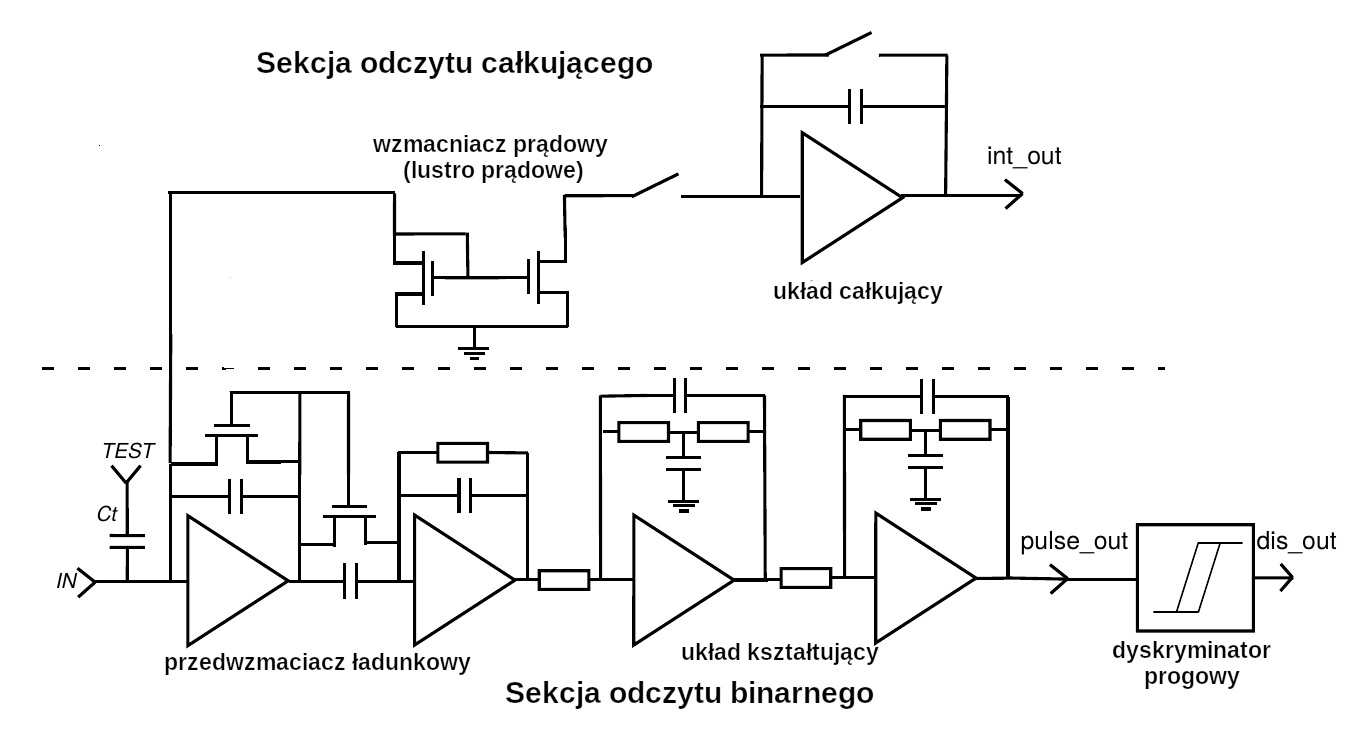
\includegraphics[width=\textwidth]{RXHDR_shaper_pl.jpg}
        \caption{Schemat blokowy pojedynczego kanału elektroniki front-end projektu RXHDR\_V1}
        \label{RXHDR schema}
\end{figure}

Poniżej prezentowane są podstawowe parametry opisujące funkcjonalnie układy binarnej architektury odczytu.

\paragraph{Krzywa-S}

Poprzez zmianę napięcia dyskryminacji w dyskryminatorze i jednoczesnym  pomiarze kolejnych impulsów detekcji możliwe jest uzyskanie widma całkowego zwanego krzywą-S. Przy założeniu mono-energetyczności sygnału równanie wyrażające zależność napięcia dyskryminacji od liczby zliczeń przybiera następującą postać:

\begin{equation}
        \label{wste krzywa s}
        S(U_{th}) = \frac{f_g}{2} * erf^{-1}(\frac{U_{th}-\overline{U_{th}}}{\sigma*\sqrt{2}})
\end{equation}
Gdzie:
\begin{description}
        \item $f_g$ - częstotliwość zdarzeń,
        \item $erf^{-1}$ - odwrotna funkcja błędu gdzie: $erf^{-1}(x) = 1 - \frac{2}{\sqrt{\pi}} \int^x_0 exp(-t^2)dt $
        \item $U_{th}$ - napięcie dyskryminatora,
        \item $\overline{U_{th}}$ - poziom dyskryminacji odpowiadający średniej amplitudzie impulsów (peak position) wartość ta pośrednio odpowiada energii sygnału, 
        \item  $\sigma$ - wartość niepewności odpowiadająca wartości szumowej układu. 
\end{description}

Przykłady takich krzywych dla różnych wartości szumów są wizualizowane na rysunku \ref{wyk s curve wstep}. Dodatkowym elementem nieuwzględnionym w wzorze są tak zwane szumy Rice’a. Pojawiają się one dla wartości napięcia dyskryminacji niższego niż średnia amplituda szumów. Stan taki powoduje zliczanie szumów jako sygnałów detektora w takiej ilość że jedynym ograniczeniem jest wydajność elektroniki \cite{wiocek doctorat}.

Dopasowanie krzywej-S do zbadanej charakterystyki układu pozwala na wyciągniecie wniosków o funkcjonowaniu kanałów na podstawie współczynników tejże zależności.   

\begin{figure}[h]
        \centering
        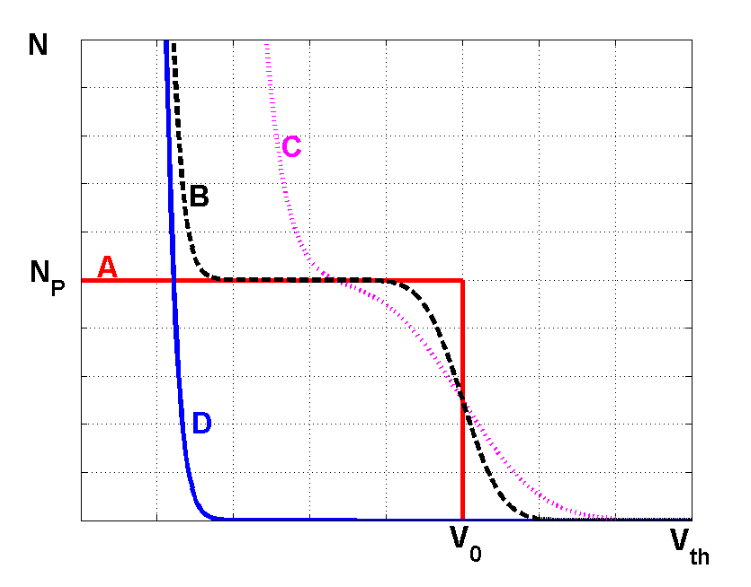
\includegraphics[height=8cm]{s_curve.png}
        \caption{Przykłady krzywych-S dla różnych wartości szumowych. A - idealny przypadek bez udziału szumów, B,C - rzeczywiste przypadki z uwzględnieniem przyczynku szumowego ($\sigma_C=2\sigma_B$), D - szum bez sygnału. \cite{wiocek doctorat}} 
        \label{wyk s curve wstep}
\end{figure}

\paragraph{RCS}
(ang. \textit{relative charge sharing})
Dodatkowym elementem nieuwzględnianym we wzorze \ref{wste krzywa s} jest efekt podziału ładunku dla detektorów pozycjoczułych. Występuje on w chwili gdy miejscem oddziaływania fotonu jest obszar między sąsiednimi segmentami detektora pozycjoczułego. Sygnał rejestrowany przez sąsiednie kanały odczytu ma poziom niższy niż ten który uzyskiwany jest tylko na jednym elemencie detekcyjnym bez podziału ładunku.
Podział ładunku powoduje powstanie dwóch osobnych sygnałów o zmniejszonej energi. Sprawia to że przy napięciu dyskryminacji dopasowanej do energii fotonu przypadek podziału ładunku dla tego fotonu nie wygeneruje binarnego sygnału zliczenia. 
%  Dla układu o dobrze dopasowanej wartości napięcia dyskryminacji taki przypadek zostałby pominięty.

Podział ładunku nie zawsze dzieli się równo między segmentami detekcji pozycjoczułej dlatego też wraz z obniżaniem napięcia dyskryminacji liniowo będzie zwiększać się liczba zliczeń impulsów o rejestrowanej niepełnej energii.~\cite{Monika mag}. 

Po uwzględnieniu tego efektu w wzorze \ref{wste krzywa s} otrzymujemy następującą równość:
\begin{equation}
        \label{wstep rcs}
        S_{RCS}(U_{th}) = (1-RCS * \frac{U_{th}}{\overline{U_{th}} - 0.5}) * S(x)
\end{equation}

Gdzie RCS to współczynnik współdzielenia ładunku a $S_{RCS}(x)$ to krzywa-S z uwzględnieniem współczynnika RCS.

Efekt ten występuje tylko przy pracy z źródłem promieniowania i stopień wpływu tego zjawiska na rezultaty wynika głównie z geometrii i umiejscowienia elementów segmentacyjnych detektora pozycjoczułego.

\paragraph{ENC}
 (ang. \textit{Equivalent Noise Charge}) ekwiwalenty ładunek szumowy jest to taka wartość ładunku, przy impulsie prądowym o kształcie delty Dirack'a, która wprowadzona na wejście przedwzmacniacza dałaby sygnał równy wartości średniokwadratowej poziomu szumów elektroniki front-end. Na podstawie dopasowanych współczynników krzywej-S można wyznaczyć ENC dla układu jako: 
 \begin{equation}
        \label{enc}
         ENC = \frac{\sigma}{K_{toru}}
 \end{equation}
 Gdzie:
 \begin{description}
        \item  $\sigma$ - wartość niepewności odpowiadająca wartości szumowej układu, 
        \item $K_{toru}$ - wzmocnienie toru odczytu.
 \end{description}
 
\noindent
Wartość wzmocnienia toru odczytu można określić jako:
\begin{equation}
        \label{k_toru}
        K_{toru} = \frac{p_{p_E}}{C_E}
\end{equation}
Gdzie:
\begin{description}
        \item  $p_{p_E}$ - (ang. peak position) próg dyskryminacji odpowiadający położeniu połówkowej wartości krzywej-S piku dla energii $E$
        \item  $C_E$ - ładunek wygenerowany poprzez depozycję energii E w układzie detektora.
\end{description}

Prezentowany powyżej wzór wzmocnienia zakłada liniowy charakter dla funkcji przenoszenia toru odczytowego i zerowy poziom napięcia niezrównoważenia dyskryminatora. W przypadku ogólnym wzmocnienie jest wartością współczynnika nachylenia stycznej do funkcji przenoszenia.

Po połączeniu wzorów \ref{enc} oraz \ref{k_toru} otrzymujemy końcowy wzór na wartość ekwiwalentnego ładunku szumowego:
\begin{equation}
        ENC = \frac{\sigma}{p_{p_E}/C_E}
\end{equation}


\subsubsection{Proces kompilacji programu na przykładzie \textit{gcc}}

Językiem rozumianym przez procesory jest kod maszynowy składający się jedynie z ciągu zer i jedynek.
Sprawia to że jest on trudny do pisania kodu i próba tworzenia w ten sposób często niesie ze sobą wiele błędów. 
Dlatego też w przeciągu lat były budowane inne języki programowania które dzięki procesowi kompilacji przetwarzają kod języka na kod maszynowy. 
Jednym z ważniejszych języków programowania stał się język \textit{c} z kompilatorem \textit{gcc - gnu c compiler}\cite{gcc}. 

Ten wysokopoziomowy język dzieli proces kompilacji na 4 części

\paragraph{Preprocesing}

Pierwszym etapem kompilacji jest preprocesing, podczas którego linie rozpoczynające się od \# są interpretowane jako komendy preprocesora.  
Za pomocą tych poleceń możemy między innymi:
\begin{itemize}
        \item Definiować zmienne - pozwala to na łatwiejszą konfigurację programu podczas fazy testów
        \item Definiować makra - ułatwiając późniejsze ponowne użycie kodu w innej części programu
        \item Warunkowo pomijać fragmenty kodu - ułatwia tworzenie różnych konfiguracji programu i redukuje ilość nie używanego kodu
        \item Wskazywać potrzebne biblioteki oraz lokalizację innych plików źródłowych.
        \item Rozwiązywać problemy kompilacyjne (header guards)
\end{itemize}
Warto dodać że wszelka logika i czynności wykonane przez prepocesor nie będą wykonywane przy każdej egzekucji programu, co może pozwolić na optymalizacje działania. 

\paragraph{Kompilacja}

Podczas tego etapu wcześniej przygotowany program zostaje przetłumaczony na język asemblera. 

Ten niskopoziomowy język jest już bardzo zależny od architektury procesora, każda z  instrukcji asemblera jest podobna do kodu maszynowemu danego procesora. 
Dlatego też analiza programu po procesie kompilacji do kodu asemblera pozwala na dokładne przewidzenie działania programu, dodatkowo
ze względu na bardzo dobrą kontrolę wykonywanych przez procesor czynności pisanie lub edytowanie kodu w asemblerze pozwala, przy odpowiednich umiejętnościach, na ostateczną optymalizację. 

Każda z poleceń asemblera składa się z dwóch części, z mnemoniki najczęściej odpowiadającej odpowiedniemu kodowi operacji procesora oraz dodatkowych danych takich jak używane rejestry lub elementy pamięci. 

\paragraph{Asemblacja}

W tym kroku przetworzony zostaje kod asemblera na język maszynowy, każda z części programu tworzy pliki z domyślnym charakterystycznym rozszerzeniem \textit{.o}.
Są to tak zwane pliki obiektowe.
Te binarne pliki już zawierają instrukcje kodu maszynowego, ale nie tworzą spójnej całości. Jest to zbiór elementów odpowiadający każdemu z użytych plików źródłowych.

\paragraph{Konsolidacja}
Konsolidator (ang. linker) program łączący wszystkie pliki obiektowe w jeden wykonywalny program. To właśnie na tym etapie dodaje się statyczne biblioteki oraz sprawdza obecność wcześniej zadeklarowanych zmiennych oraz upewnia się że nie pojawia się konflikt oznaczeń. Po zakończeniu tego procesu otrzymujemy gotowy program. 


\subsubsection{Czas wykonalności programu}

By wyznaczyć czas konieczny na wykonanie programu lub fragmentu programu można użyć prawa wydajności procesora\cite{arch}:

\begin{equation}
        \label{Iron Law}
        \frac{Czas}{Program} =  \frac{Instrukcje}{Program} * \frac{Cykle}{Instrukcje} * \frac{Czas}{Cykl}
\end{equation}

Elementy tego równania są zależne od różnych elementów układu komputerowego:
\begin{description}
        \item $\frac{Instrukcje}{Program}$ - powiązany z językiem programowania, optymalizacją kompilatora oraz długością programu. 
        \item $\frac{Cykle}{Instrukcje}$ - Zależy od mikroarchitektury komputera oraz modelu programowego procesora.
        \item $\frac{Czas}{Cykl}$ -  zależny od prędkości taktowania procesora i technologi chipu. 
\end{description} 


W celu obliczenia czasu wykonania pojedyńczego cyklu ($\frac{Czas}{Cykl}$), dla architektury w której jeden cykl zegara głównego to jeden cykl procesora, można skorzystać z równości:
\begin{equation}
        \label{Cykli w sec}
        t_c [s]= \frac{1}{T [Hz]}
\end{equation} 
Gdzie:\\
\indent $t_c$ - czas pojedynczego cyklu \\
\indent $T$ - taktowanie procesora w Hz

\subsubsection{Potokowość}

W celu ograniczenia ilości cykli przypadających na jedną instrukcję używa się technologi potokowości. 
Oznacza to że pojedynczą instrukcję dzielimy na mniejsze części i pozwalamy zasobom które odpowiadają za wykonanie tych części pracować nad następnym zadaniem zanim całość instrukcji zostanie wykonana.

Przykładowy podział instrukcji może wyglądać następująco:
\begin{enumerate}
        \item IF - (instruction feach) - pobranie instrukcji
        \item ID - (instruction decode) -  zdekodowanie instrukcji
        \item EX - (execute) - wykonanie instrukcji - arytmetyka
        \item MEM - (memory acces) - dostęp do pamięci
        \item WB - (write back) - zapisanie wyniku
\end{enumerate}

Dzięki takiemu rozbiciu w idealnym przypadku możemy osiągnąć architekturę pozwalającą wykonywać każdą instrukcję w jednym cyklu procesora. 

\begin{table}{}
        \centering
        \caption{Przykład pracy procesora z wykorzystaniem potokowości w idealnym przypadku.}
        \label{pipelining}
        \begin{tabular}{lcccccccc}
                Czas & $t_0$&$t_1$&$t_2$&$t_3$&$t_4$&$t_5$&$t_6$&$t_7$ \\ \hline
                Instrukcja 1 & IF & ID & EX & MEM & WB &    & \\
                Instrukcja 2 &    & IF & ID & EX & MEM & WB & \\
                Instrukcja 3 &    &    & IF & ID & EX & MEM & WB \\
                Instrukcja 4 &    &    &    & IF & ID & EX & MEM & WB
        \end{tabular}
\end{table}


Taki przypadek jest wizualizowany w tabeli \ref{pipelining}. Jak widać żaden z zasobów nie jest wykorzystywany równocześnie przez dwie instrukcje.
Dodatkowo tabela \ref{pipelining} pokazuje że każda następna instrukcja jest wykonywana w kolejnym czasie $t$. 
Czas $t$ jest równy czasowi najdłuższego etapu z dodatkiem czasu wymaganego przez elektronikę zarządzającą potokowością \cite{arch}.
Równość ta może być zapisana wzorem:
\begin{equation}
        t = T_{e_{max}} + T_{+}
\end{equation}
Gdzie:
        $t$ - minimalny czas cyklu procesora \\
        $T_{e_{max}}$ - czas konieczny na wykonanie najdłuższego etapu \\
        $T_{+}$ - dodatkowy czas wymagany przez rejestry \\


Powyższy przykład pokazuje jedynie pięcio-etapową potokowość jednak procesory komercyjne stosują różne rozwiązania. Przykładowo SMART SAM3X/A stosuje trój etapową potokowość\cite{datasheet} a mikroarchitektura Intel'a o nazwie Nehalem może zawierać 20 - 24 etapów\cite{pipelining intel}.

Jednak podczas rozwiązań tego typu nie zawsze trafimy na sytuacje kiedy pojedynczy cykl przypada dla pojedynczej instrukcji. 
Rozwiązanie potokowości przynosi ze sobą pewne zagrożenia. Poniżej znajdują się krótkie opisy takich sytuacji. 

\begin{itemize}
        \item Dane - sytuacja gdy instrukcja wymaga informacji wytworzonej przez instrukcję ciągle realizowaną w potoku. 
        \item Zasoby - gdy polecenie wymaga użycia zasobu (RAM, PC lub ALU) który aktualnie jest używany przez inny etap potoku. 
        \item Rozwidlenia - Sytuacje gdy program zmienia swój naturalny bieg, czy to przez przerwanie systemowe czy skoki warunkowe. 
\end{itemize}

Jest wiele rozwiązań pozwalających zmniejszyć ilość wystąpień takich sytuacji lub ograniczyć straty powodowane przez takie sytuacje, jednak nadal konieczne są zastosowania chwilowego zatrzymania elementów potoku, lub w najgorszym wypadku całkowitego oczyszczenia.
Powoduje to że niektóre z instrukcji mogą wymagać większej ilości cykli niż jeden. Jednakże przy zastosowaniu takich technik jak
\textit{Out-of-order execution}, \textit{branch prediction} oraz programowanie równoległe  sprawia że przewidzenie czasu koniecznego na wykonanie programu metodami analitycznymi staje się trudne . 
Z tego też powodu w tym celu stosuje się metody statystyczne oraz testowanie wzorcowe. 

\subsubsection{Programowanie wielowątkowe}

Wątek (ang. \textit{thread}) jest to część programu która może być oddzielnie zarządzana przez dyspozytor (ang. \textit{scheduler}). 
Pozwala to na wykonywanie wielu wątków równocześnie w przypadku procesorów wielowątkowych lub częste zmiany uwagi między zadaniami w procesorach jednowątkowych.
W przeciwieństwie do osobnych procesów wątki dzielą wspólną przestrzeń adresową (korzystają z tych samych danych) oraz współdzielą zasoby systemowe.

Użycie metod programowania wielowątkowego niesie ze sobą wiele zalet:
\begin{itemize}
        \item Oprogramowanie korzystające z interfejsu użytkownika (GUI - \textit{grafic user interface}) może pozostać gotowe na nowe informacje nawet podczas wykonywania trudnych obliczeń jeżeli zadanie odpowiedzialne za UI (ang. User interface - interfejs użytkownika) będzie osobnym wątkiem niż ten wykonujący obliczenia.
        \item Ponieważ zasoby są współdzielone między wątkami podejście wielowątkowe może być bardziej oszczędne w zasoby w porównaniu z użyciem osobnych procesów, które wymagałoby przekopiowania danych.
        \item Program może działać szybciej i z mniejszym opóźnieniem, dzięki programowaniu z użyciem większej ilości wątków, ponieważ pozwala to na lepsze wykorzystanie popularnej architektury wielordzeniowej procesorów komercyjnych. 
        \item Każda część programu którego obliczenia mogą zostać wykonane równolegle może zyskać na szybkości przy użyciu wielowątkowego podejścia zgodnie z prawem Amdahala \cite{arch}. 
        Jednak dla przypadku obliczeń które nie pozwalają na równoległe wyliczenia, proces tworzenia wątków oraz wymaganie czekania na zwolnienie zasobów może spowodować że prędkość programu się obniży.
\end{itemize}
Jak widać użycie programowania wielowątkowego niesie ze sobą wiele korzyści,
jednak wraz z zaletami tego rozwiązania spotykamy się z pewnymi zagrożeniami i wymaganiami.

\paragraph{Synchronizacja i współdzielenie zasobów.}

Tak jak było to wcześniej opisane w przeciwieństwie do rozpoczęcia nowego procesu na nowe obliczenia, programowanie wielowątkowe pozwala na kontynuowanie obliczeń bez kopiowania zasobów. 
Powoduje to jednak, że wymagane są sposoby sygnalizacji między wątkami oraz sposoby ochrony zasobów przed równoczesnym dostępem przez więcej niż jedno zadanie. 
Ta potrzeba spowodowała tworzenie powtarzalnych struktur które są implementowane w najpopularniejszych językach programowania. 
Poniżej znajduje się ich krótki opis bez skupienia na specyfice którejkolwiek z implementacji. 
\begin{itemize}
        \item mutex/zamek (ang. \textit{lock}) - obiekt który ma dwa stany zablokowany/otwarty.
        Kiedy wątek próbuje zablokować mutex/zamek który już jest zablokowany powoduje to przejście wątku w stan czekania aż do chwili odblokowania przez zadanie które pierwotnie zablokowało mutex.
        Daje to możliwość wykorzystania tej struktury w celu ochrony zasobu. Przed rozpoczęciem zadania który wymaga wyłączności blokujemy mutex dając sygnał korzystania z zasobu do którego ten lock należy. 
        Po zakończeniu obliczeń zwalniamy/otwieramy mutex pozwalając pracować innym wątkom. Obiekt ten może być jedynie zwolniony przez wątek który go zablokował. 
        W ten właśnie sposób unika się równoczesnego korzystania z zasobów. 
        \item semafor (ang. \textit{semaphore}) - zasada działania jest podobna do mutexu jednak w przeciwieństwie do wcześniej wymienionej struktury semafor może być odblokowywany przez inne wątki niż te które zablokowały obiekt. Dodatkowo w częstej implementacji semafor może mieć więcej niż jeden stopień blokady. 
        Jest on przydatny w przypadku potrzeby synchronizacji obliczeń. Jeden z wątków może zablokować semafor oznajmiając że skończył swoje obliczenia i oczekuje na wynik z równoległych obliczeń, a inny wątek po zakończeniu swojej części może odblokować semafor. 
        \item monitor - obiekt ten ma zapisaną listę aktualnie używanych zasobów i jeżeli wątek próbuje (korzystając z funkcji monitora) skorzystać z zasobu spowoduje to przejście w stan wstrzymania wątku aż do zwolnienia zasobu. 
        Monitor zapewnia funkcjonalność mutex/lock dla dowolnego zasobu, jednak korzystanie z tej funkcjonalności sprawia trudności w tworzeniu fragmentów kodu który jest krytyczny gdyż w takim przypadku konieczne byłoby skorzystanie z monitora w celu zablokowania każdego z zasobów z osobna podczas gdy mutex/lock może być odpowiedzialny za wiele zasobów jednocześnie.   
\end{itemize} 

Korzystanie z funkcji synchronizujących jest konieczne w celu uniknięcia błędów występujących w wyniku korzystania z programowania wielowątkowego. Poniżej wymienione są najpopularniejsze zagrożenia  wynikające z korzystania z metod obliczeń równoległych. 

\paragraph{Sytuacja wyścigu (ang. \textit{race condition})}

\begin{figure}[t]
        \centering
        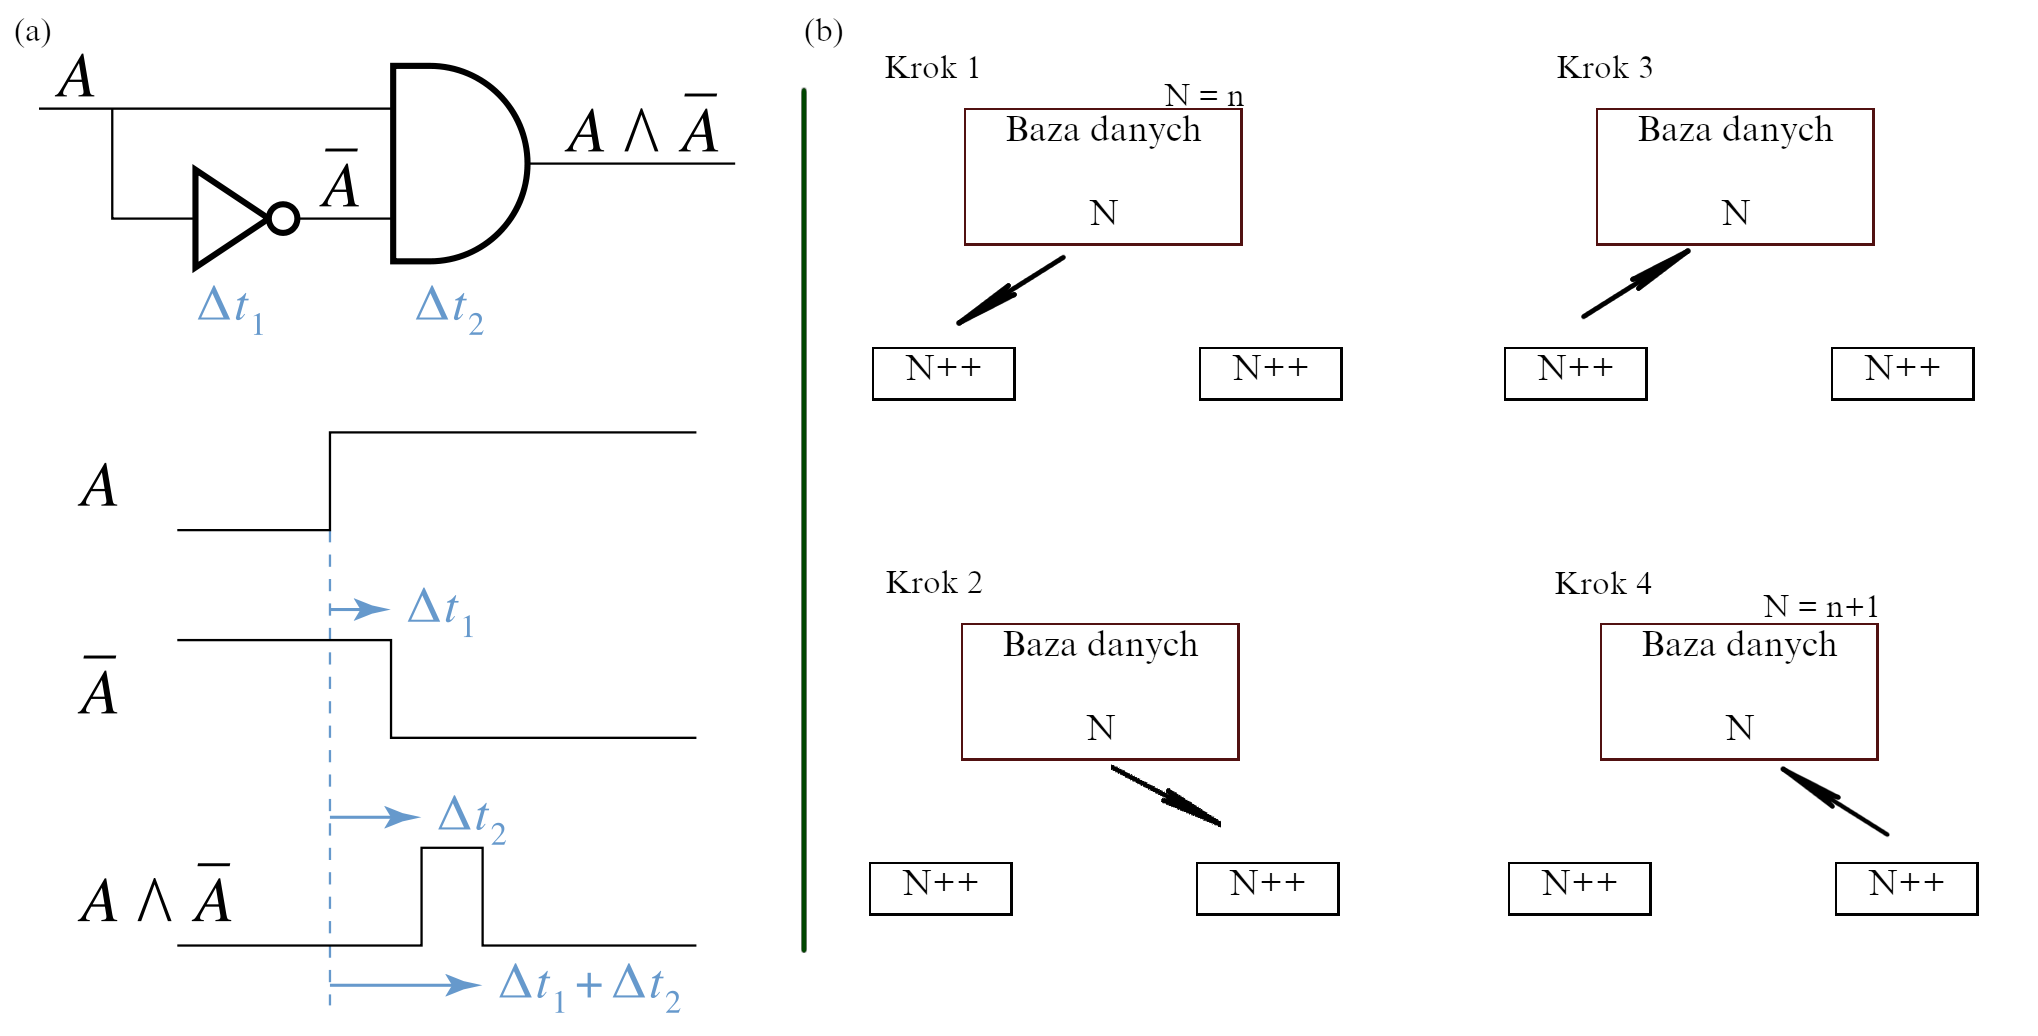
\includegraphics[width = \textwidth]{race_condition.png}
        \caption{Schematy układów w których występuje hazard (ang. \textit{race condition}). Po lewej \textit{(a)} przykład układu elektronicznego a po prawej \textit{{b}} schemat działania programu wielowątkowego. }
        \label{race condition}
\end{figure}

W elektronice sytuacja wyścigu to hazard spowodowany przez czas propagacji elementów układu powodujący niezamierzane efekty. Przykład układu elektronicznego w którym występuje takowy hazard jest wizualizowany na rysunku \ref{race condition}(a). 
Sytuacje wyścigu dzielą się na statyczne i dynamiczne. Statyczne to takie w których obserwujemy zmianę na wyjściu w chwili gdy dla układów o zerowej propagacji elementów spodziewalibyśmy się niezmienionego stanu.
W hazardzie dynamicznym spotykamy się z odwrotną sytuacją. 

W przypadku programowania wielowątkowego tego typu hazard nie jest powodowany przez czas propagacji elementów lecz przez nieznany czas i kolejność wykonywania operacji przez równolegle pracujące wątki. Przykład schematu programu dla takiego przypadku znajduje się na rysunku \ref{race condition}(b). Schemat przedstawia prostą bazę danych i dwa wątki mające za zadanie podniesienie wartości zmiennej \textit{N} o jeden.
Prosty proces zmiany zmiennej składa się z trzech oddzielnych części, pobranie wartości zmiennej, zwiększenie wartości oraz ponowne zapisanie zmiennej w pamięci. 
Dla podanego przykładu w typowym przebiegu gdy obydwa wątki zwiększą wartość zmiennej o 1 spodziewany jest wynik $N = n+2$. Jednak rzadkim przypadku może zaistnieć sytuacja że drugi wątek pobierze wartość N do obliczeń przed zapisaniem wyniku z pierwszej operacji. Spowoduje to trudny do odnalezienia i odtworzenia błąd sprawiający że zignorowane zostają obliczenia wątku który pierwszy pobrał wartość, zatem końcowy wynik będzie równy $N = n+1$.
Jest to jeden z powodów dlaczego zabezpiecza się zasoby za pomocą muteksów lub semaforów. 

Mimo sposobów na unikanie takich sytuacji programowanie wielowątkowe wymaga dużej staranności a potencjalne błędy mogą pozostawać ukryte nawet latami. To też jest powód dla którego nie należy nadużywać takich rozwiązań jeżeli mogą zostać pominięte\cite{multi thread problem}.
\paragraph{Zakleszczenie.}

Zakleszczenie (ang. \textit{deadlock}) to sytuacja gdy dwie operacje czekają na siebie wzajemnie więc żadna z nich nie może się zakończyć. 
Zakleszczenie może występować w procesach, wątkach jak i również w świecie fizycznym przykładowo w ruchu drogowym podczas blokady ronda w korku drogowym.  
Prostym przykładem takiej sytuacji jest chwila gdy dwa procesy w celu przeprowadzenia obliczeń potrzebują dwóch muteksów i w chwili gdy każdy z nich zablokuje jeden z nich przechodzą w stan wstrzymania oczekując na zwolnienie tego trzymanego przez konkurujący proces. 

 Kiedykolwiek występuje graf cykliczny zapotrzebowania zasobów deadlock może zaistnieć. 
 Powoduje to że jest to trudna sytuacja do przewidzenia w bardziej rozbudowanych programach.

W celu uniknięcia takiej sytuacji można wprowadzić pewne środki zapobiegawcze\cite{coffman}:
\begin{itemize}
        \item Proces/wątek blokuje zasoby dopiero kiedy wszystkie są dostępne. Jest to mało optymalne rozwiązanie i może spowodować że operacja nigdy nie zostanie przeprowadzona
        \item Ustalenie mechanizmu wywłaszczania zasobów oraz hierarchii dostępu. 
        \item Przed przejściem w stan oczekiwania proces może zwolnić wszystkie przetrzymywane zasoby. 
        \item Usunięcie wymagania wyłączności. Jeżeli zasób może być używany przez wiele wątków/procesów jednocześnie to nie należy go blokować.  
        \item Projektowanie programu tak by proces/wątek wymagał jednocześnie dostępu jedynie do jednego zasobu na raz. 
\end{itemize} 

Jest to kolejny powód dla którego należy bardzo rozsądnie podchodzić do projektowania programu przy decyzji programowania wielowątkowego oraz nie nadużywać tego podejścia w sytuacjach gdy jest to niekonieczne\cite{multi thread problem}. 

\subsubsection{Otwarte formaty danych}

Pliki o otwartych formatach danych to takie pliki tekstowe których metadane oraz semantyka jest ogólnie dostępna. 
Celem tych plików jest łatwość interpretacji zarówno przez człowieka jak i maszynę. 
Oznacza to że nie tylko są to formaty które są często implementowane w wielu programach, ale również umożliwiają ręczną manipulację danymi przez użytkownika.  
Poniżej znajdują się krótkie opisy najpopularniejszych formatów.

\paragraph{CSV}
(ang. \textit{Comma Seperated Values}, wartości dzielone przecinkami) jest to prosty format plików w którym zgodnie z nazwą każda z wartości jest oddzielana przecinkiem od kolejnej. Wartości dzielą się na rekordy oddzielane znakami końca linii CRLF oraz wartości oddzielane przecinkami. Zamiast przecinków mogą być używane znaki specjalne jak średniki lub tabulatury chociaż jest to niezalecane. Jeżeli plik z danymi zawiera tablicę to ilość wartości powinna być jednakowa w każdym z rekordów. 

\paragraph{XML}
(ang. \textit{Extensible Markup Language}) jest to uniwersalny język znaków służący do przenoszenia danych. Jego skupieniem była łatwość w pisaniu programów interpretujących ten standard.
Jest to język na podstawie którego stworzono wiele ważnych pochodnych formatów takich jak Microsoft Office XML formats, Trusted Data Format i HTML5.

Poniżej znajduje się prosty przykład takiego dokumentu:
\begin{kod}
        \lstinputlisting[language=XML]{code_source/XML.xml}
        \caption{Schematyczny przykład zawartości pliku napisanego w języku XML}
        \label{XML code}
\end{kod}

Dokument XML składa się z elementów, atrybutów oraz tagów. 
Tagi znajdują się między symbolami < > oraz każdy z nich wymaga zamknięcia przez tag o tej samej nazwie rozpoczynając się od znaku \textbackslash.
Atrybuty to pary wartość klucz znajdujące się między symbolami < > gdzie wartość zawsze musi być zawarta między znakami ".
Wartości to tekst lub kolejne elementy znajdujące się między tagami. 
Pierwsza linia to opcjonalny prolog zawierający informację o wersji XML oraz typie kodowania.  
Dokument XML musi zawierać element początkowy, w przykładowym kodzie \ref{XML code} jest to tag <root>.

\paragraph{JSON }
(ang. \textit{JavaScript Object Notation}) mimo że nie jest on standardem otwartych plików danych, lecz formą języka JavaScript to spełnia warunki czytelności przez człowieka jak i maszynę. 
Forma obiektu w tym języku stała się w przeciągu lat popularnym sposobem na przekazywanie danych między aplikacjami. Stało się tak ze względu na prostotę semantyki oraz uniwersalność. 

Każdy obiekt JSON zaczyna się symbolem \{ i kończy \} każda z wartości składa się z pary atrybut wartość przedzielona dwukropkiem, a każda z kolejnych par oddziela się przecinkiem. Typami wartości są:
\begin{itemize}
        \item liczba, 
        \item tekstowy typ danych (ang. string),
        \item logiczny typ danych,
        \item tablica - zaczyna się od [ kończy na ],
        \item obiekt,
        \item wartość pusta - null. 
\end{itemize}

Format ten wspierany jest przez wiele języków między innymi C, C++, C\#, Java, JavaScript, Perl, Python\cite{json}.

\subsubsection{Rejestr przesuwny}
Rejestr to taki układ elektroniczny którego celem jest przechowywanie oraz umożliwienie dostępu do danych. Funkcja ta jest podobna do funkcji pamięci jednak w przeciwieństwie do pamięci rejestry mogą mieć dodatkową funkcję sprzętową.
Przykładowo rejestry mogą służyć w celu komunikacji między kodem a urządzeniami wejścia/wyjścia.

Specjalnym przykładem rejestru jest rejestr przesuwny którego dane, przy sygnale z zegara, będą przekazywane do kolejnego miejsca przetrzymywania informacji w ściśle określonym kierunku.  
Najczęściej rejestry przesuwne są skonstruowane jako kaskada przerzutników gdzie wejście danych kolejnego przerzutnika jest połączone z wyjściem poprzedniego.

Istnieją 4 typy rejestrów przesuwnych różniących się ze względu na sposób wprowadzania i odbioru danych:
\begin{itemize}
        \item szeregowo-szeregowy,
        \item równolegle-szeregowy,
        \item szeregowo-równoległy,
        \item równolegle-równoległy zwany rejestrem buforowym.
\end{itemize} 
